\documentclass[aspectratio=169]{beamer}

% ---------- ENCODING & FONTS ----------
\usepackage[utf8]{inputenc}
\usepackage[T1]{fontenc}

% ---------- THEME & LOOK ----------
\usetheme{Madrid}
\usecolortheme{seahorse}
\usefonttheme{professionalfonts}
\setbeamertemplate{navigation symbols}{}
\setbeamercovered{transparent}
\setbeamertemplate{itemize items}[circle]
\setbeamertemplate{enumerate items}[default]
\setlength{\parskip}{0.25em}

% ---------- COLORS ----------
% Beamer already loads xcolor, so we just define our colors
\definecolor{accent}{RGB}{0,92,184}
\definecolor{soft}{RGB}{233,244,255}
\definecolor{lightred}{RGB}{245,210,210}
\setbeamercolor{structure}{fg=accent}
\setbeamercolor{title}{fg=white,bg=accent}
\setbeamercolor{frametitle}{fg=accent}
\setbeamercolor{block title}{bg=accent!12,fg=accent}
\setbeamercolor{block body}{bg=soft}

% ---------- PACKAGES ----------
\usepackage{booktabs}
\usepackage{amsmath, amssymb}
\usepackage{array}
\usepackage{multirow}
\usepackage{hyperref}
\hypersetup{colorlinks=true,linkcolor=accent,urlcolor=accent}

% ---------- SAFE TRANSITION FALLBACK ----------
\makeatletter
\@ifundefined{transfade}{\newcommand{\transfade}[1][]{}}{}
\makeatother

% ---------- PLACEHOLDER BOX FOR FIGURES ----------
\newcommand{\placeholderbox}[2][0.82\linewidth]{%
  \begin{center}
    \fbox{\begin{minipage}[c][0.46\textheight][c]{#1}
      \centering \vspace{0.3em}
      \textbf{#2}\\[0.6em]
      \emph{Insert figure/diagram here later.}
    \end{minipage}}
  \end{center}
}


% ---------- TITLE ----------
\title{\textbf{Aggregate Demand and Aggregate Supply Analysis \vspace{.5cm}\\  }}
\subtitle{ {\large ECON 101 - Macroeconomics}}
%\institute{UNBC}
\author{Muhebullah Karimzada}
\date{Winter 2026}



\begin{document}

% ============================================================
% TITLE
% ============================================================
\begin{frame}[plain]
  \titlepage
\end{frame}

% ============================================================
\begin{frame}{Chapter Outline}
\transfade
\begin{itemize}[<+->]
  \item \textbf{9.1} Aggregate Demand
  \item \textbf{9.2} Aggregate Supply
  \item \textbf{9.3} Macroeconomic Equilibrium in the Long Run and the Short Run
\end{itemize}
\end{frame}

% ============================================================
\section{9.1 Aggregate Demand}
% ============================================================

\begin{frame}{9.1 Learning Objective}
\transfade
\begin{block}{Goal}
Identify the determinants of aggregate demand and distinguish between a movement along the AD curve and a shift of the curve.
\end{block}
\begin{itemize}[<+->]
  \item Real GDP has four components:
  \begin{itemize}[<+->]
    \item Consumption \((C)\)
    \item Investment \((I)\)
    \item Government purchases \((G)\)
    \item Net exports \((NX)\)
  \end{itemize}
  \item Adding these gives:
  \[
    Y = C + I + G + NX.
  \]
  \item In this chapter we treat each component as a \textbf{function of the price level and other variables} and use them to build the \textbf{aggregate demand curve}.
\end{itemize}
\end{frame}

\begin{frame}{Aggregate Demand and Aggregate Supply Model}
\transfade
\begin{itemize}[<+->]
  \item We have already modeled:
  \begin{itemize}[<+->]
    \item long-run economic growth, and
    \item short-run output determination using the AE model.
  \end{itemize}
  \item Now we extend our short-run model to understand:
  \begin{itemize}[<+->]
    \item why real GDP, employment, and the price level fluctuate together.
  \end{itemize}
  \item \textbf{Aggregate demand and aggregate supply model:}
  \begin{itemize}[<+->]
    \item explains short-run fluctuations in real GDP and the price level.
  \end{itemize}
\end{itemize}
\end{frame}

\begin{frame}{Figure 9.1 -- Aggregate Demand and Aggregate Supply }

\centering
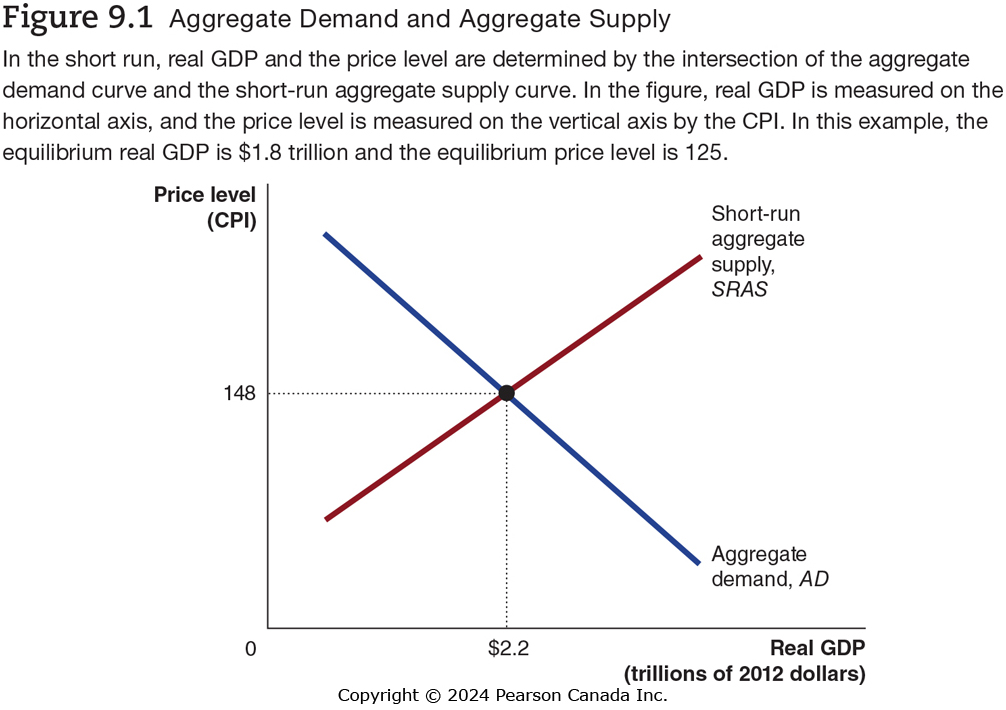
\includegraphics[width=0.7\linewidth]{Fig09-001}
\end{frame}

\begin{frame}{AD and SRAS: Basic Definitions}
\transfade
\begin{itemize}[<+->]
  \item \textbf{Aggregate demand (AD) curve:}
  \begin{itemize}[<+->]
    \item Shows the relationship between the price level and the quantity of real GDP demanded by:
    \begin{itemize}[<+->]
      \item households, firms, the government, and the foreign sector.
    \end{itemize}
  \end{itemize}
  \item \textbf{Short-run aggregate supply (SRAS) curve:}
  \begin{itemize}[<+->]
    \item Shows the relationship in the short run between the price level and the quantity of real GDP supplied by firms.
  \end{itemize}
  \item The intersection of AD and SRAS determines the \textbf{short-run macroeconomic equilibrium}.
\end{itemize}
\end{frame}

% ------------------------------------------------------------
% Why AD Slopes Down
% ------------------------------------------------------------

\begin{frame}{Why the Aggregate Demand Curve Slopes Down}
\transfade
\begin{itemize}[<+->]
  \item As the \textbf{price level} rises:
  \begin{itemize}[<+->]
    \item households feel poorer,
    \item interest rates tend to rise,
    \item domestic goods become more expensive relative to foreign goods.
  \end{itemize}
  \item Each of these channels reduces one or more components of real GDP:
  \begin{itemize}[<+->]
    \item \(C\) (consumption),
    \item \(I\) (investment),
    \item \(NX\) (net exports).
  \end{itemize}
  \item Result: a \textbf{higher} price level is associated with a \textbf{smaller} quantity of real GDP demanded.
\end{itemize}
\end{frame}

\begin{frame}{The Wealth Effect: Price Level and Consumption}
\transfade
\begin{itemize}[<+->]
  \item Household consumption is mostly determined by income, but also by \textbf{wealth}.
  \item Some household wealth is held in \textbf{nominal assets} (cash, bank deposits, bonds).
  \item When the price level rises:
  \begin{itemize}[<+->]
    \item the \textbf{real value} of these nominal assets falls,
    \item households feel poorer and reduce consumption.
  \end{itemize}
  \item Implication:
  \begin{itemize}[<+->]
    \item \alert{Higher price level} \(\Rightarrow\) \alert{lower consumption}.
  \end{itemize}
\end{itemize}
\end{frame}

\begin{frame}{The Interest-Rate Effect: Price Level and Investment}
\transfade
\begin{itemize}[<+->]
  \item When the price level rises:
  \begin{itemize}[<+->]
    \item households and firms need more money to buy and sell goods and services.
  \end{itemize}
  \item They may:
  \begin{itemize}[<+->]
    \item borrow more,
    \item withdraw funds from banks,
    \item sell financial assets such as bonds.
  \end{itemize}
  \item This extra demand for money pushes up the \textbf{interest rate}:
  \begin{itemize}[<+->]
    \item Higher interest rates discourage borrowing,
    \item which reduces investment spending.
  \end{itemize}
  \item Implication:
  \begin{itemize}[<+->]
    \item \alert{Higher price level} \(\Rightarrow\) \alert{lower investment}.
  \end{itemize}
\end{itemize}
\end{frame}

\begin{frame}{The International-Trade Effect: Price Level and Net Exports}
\transfade
\begin{itemize}[<+->]
  \item When Canadian price levels rise:
  \begin{itemize}[<+->]
    \item Canadian goods become more expensive relative to foreign goods.
  \end{itemize}
  \item Consequences:
  \begin{itemize}[<+->]
    \item Exports fall (foreigners buy fewer Canadian goods),
    \item Imports rise (Canadians buy more foreign goods).
  \end{itemize}
  \item Net exports \(NX = X - M\) therefore fall.
  \item Implication:
  \begin{itemize}[<+->]
    \item \alert{Higher price level} \(\Rightarrow\) \alert{lower net exports}.
  \end{itemize}
\end{itemize}
\end{frame}

\begin{frame}{Summary: Why AD Slopes Down}
\transfade
\begin{itemize}[<+->]
  \item Each effect links a higher price level to lower spending:
  \begin{itemize}[<+->]
    \item Wealth effect \(\Rightarrow\) lower \(C\),
    \item Interest-rate effect \(\Rightarrow\) lower \(I\),
    \item International-trade effect \(\Rightarrow\) lower \(NX\).
  \end{itemize}
  \item Together, these effects imply:
  \begin{itemize}[<+->]
    \item A downward-sloping \textbf{aggregate demand curve}.
  \end{itemize}
\end{itemize}
\end{frame}

% ------------------------------------------------------------
% Shifts vs Movements along AD
% ------------------------------------------------------------

\begin{frame}{Movements Along vs. Shifts of the AD Curve}
\transfade
\begin{itemize}[<+->]
  \item The AD curve shows the relationship between the \textbf{price level} and real GDP demanded, \textbf{holding everything else constant}.
  \item \textbf{Movement along AD:}
  \begin{itemize}[<+->]
    \item Caused by a change in the price level itself,
    \item not by a change in any component of spending.
  \end{itemize}
  \item \textbf{Shift of AD:}
  \begin{itemize}[<+->]
    \item Caused by a change in \(C\), \(I\), \(G\), or \(NX\) from any source \emph{other than} the price level.
  \end{itemize}
\end{itemize}
\end{frame}

% ------------------------------------------------------------
% Table 9.1 Variables That Shift AD
% ------------------------------------------------------------

\begin{frame}{Table 9.1 -- Variables That Shift the AD Curve (1 of 4)}
\transfade
\begin{block}{Government Policy: Monetary Policy}
\end{block}
\begin{itemize}[<+->]
  \item \textbf{Monetary policy:}
  \begin{itemize}[<+->]
    \item Actions the central bank (e.g., the Bank of Canada) takes to manage the money supply and interest rates to pursue macroeconomic objectives.
  \end{itemize}
\end{itemize}
\begin{table}[h]
\centering
\begin{tabular}{p{0.4\linewidth} p{0.5\linewidth}}
\toprule
\textbf{Change} & \textbf{Effect on AD} \\
\midrule
Increase in interest rates & Reduces investment and some consumption; \textbf{AD shifts left}. \\
Decrease in interest rates & Increases investment and some consumption; \textbf{AD shifts right}. \\
\bottomrule
\end{tabular}
\end{table}
\end{frame}

\begin{frame}{Table 9.1 -- Variables That Shift the AD Curve (2 of 4)}
\transfade
\begin{block}{Government Policy: Fiscal Policy}
\end{block}
\begin{itemize}[<+->]
  \item \textbf{Fiscal policy:}
  \begin{itemize}[<+->]
    \item Changes in federal taxes and purchases intended to achieve macroeconomic objectives.
  \end{itemize}
\end{itemize}
\begin{table}[h]
\centering
\begin{tabular}{p{0.45\linewidth} p{0.45\linewidth}}
\toprule
\textbf{Change} & \textbf{Effect on AD} \\
\midrule
Increase in personal income taxes & Reduces disposable income and consumption; \textbf{AD shifts left}. \\
Decrease in personal income taxes & Raises disposable income and consumption; \textbf{AD shifts right}. \\
Increase in government purchases & Directly raises G; \textbf{AD shifts right}. \\
Decrease in government purchases & Directly lowers G; \textbf{AD shifts left}. \\
Increase in business taxes & Reduces investment; \textbf{AD shifts left}. \\
Decrease in business taxes & Increases investment; \textbf{AD shifts right}. \\
\bottomrule
\end{tabular}
\end{table}
\end{frame}

\begin{frame}{Table 9.1 -- Variables That Shift the AD Curve (3 of 4)}
\transfade
\begin{block}{Changes in Expectations}
\end{block}
\begin{itemize}[<+->]
  \item Households and firms may become more optimistic or pessimistic about the future.
\end{itemize}
\begin{table}[h]
\centering
\begin{tabular}{p{0.45\linewidth} p{0.45\linewidth}}
\toprule
\textbf{Change} & \textbf{Effect on AD} \\
\midrule
Households expect higher future incomes & Increases current consumption; \textbf{AD shifts right}. \\
Households expect lower future incomes & Decreases current consumption; \textbf{AD shifts left}. \\
Firms expect higher future profitability & Increases investment; \textbf{AD shifts right}. \\
Firms expect lower future profitability & Reduces investment; \textbf{AD shifts left}. \\
\bottomrule
\end{tabular}
\end{table}
\end{frame}

\begin{frame}{Table 9.1 -- Variables That Shift the AD Curve (4 of 4)}
\transfade
\begin{block}{Changes in Foreign Variables}
\end{block}
\begin{table}[h]
\centering
\begin{tabular}{p{0.45\linewidth} p{0.45\linewidth}}
\toprule
\textbf{Change} & \textbf{Effect on AD} \\
\midrule
Domestic GDP growth rate rises relative to other countries & Imports rise faster than exports; net exports fall; \textbf{AD shifts left}. \\
Domestic GDP growth rate falls relative to other countries & Imports grow slowly, exports may rise; net exports increase; \textbf{AD shifts right}. \\
Increase in the value of the Canadian dollar (appreciation) & Canadian exports become more expensive; imports cheaper; net exports fall; \textbf{AD shifts left}. \\
Decrease in the value of the Canadian dollar (depreciation) & Canadian exports cheaper; imports more expensive; net exports rise; \textbf{AD shifts right}. \\
\bottomrule
\end{tabular}
\end{table}
\end{frame}

% ============================================================
\section{9.2 Aggregate Supply}
% ============================================================

\begin{frame}{9.2 Learning Objective}
\transfade
\begin{block}{Goal}
Identify the determinants of aggregate supply and distinguish between a movement along the SRAS curve and a shift of the curve.
\end{block}
\begin{itemize}[<+->]
  \item \textbf{Aggregate supply} refers to the quantity of goods and services that firms are willing and able to supply.
  \item The relationship between this quantity and the price level differs:
  \begin{itemize}[<+->]
    \item in the \textbf{long run}, and
    \item in the \textbf{short run}.
  \end{itemize}
  \item We develop both a long-run and a short-run aggregate supply curve.
\end{itemize}
\end{frame}

\begin{frame}{Long-Run Aggregate Supply (LRAS)}
\transfade
\begin{itemize}[<+->]
  \item \textbf{Long-run aggregate supply (LRAS) curve:}
  \begin{itemize}[<+->]
    \item Shows the relationship in the long run between the price level and the quantity of real GDP supplied.
  \end{itemize}
  \item In the long run, real GDP is determined by:
  \begin{itemize}[<+->]
    \item number of workers,
    \item level of technology,
    \item capital stock (factories, machinery, equipment).
  \end{itemize}
  \item These determinants are not affected by the price level.
  \item Therefore, \textbf{LRAS is a vertical line} at \textbf{potential (full-employment) GDP}.
\end{itemize}
\end{frame}

\begin{frame}{Figure 9.2 -- Long-Run Aggregate Supply Curve}
\centering
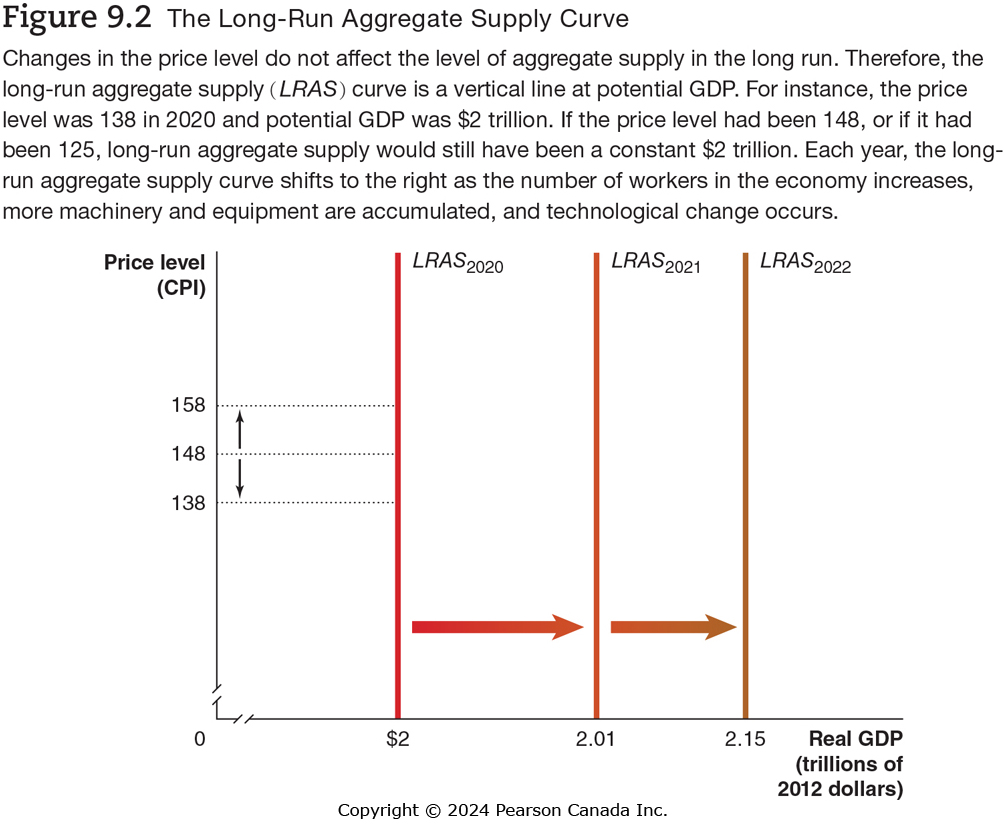
\includegraphics[width=0.6\linewidth]{Fig09-002}
\end{frame}

\begin{frame}{Short-Run Aggregate Supply (SRAS)}
\transfade
\begin{itemize}[<+->]
  \item \textbf{Short-run aggregate supply (SRAS) curve:}
  \begin{itemize}[<+->]
    \item Shows the relationship in the short run between the price level and the quantity of real GDP supplied by firms.
  \end{itemize}
  \item Unlike LRAS, the SRAS curve is \textbf{upward sloping}.
  \item Why?
  \begin{itemize}[<+->]
    \item As prices of final goods and services rise,
    \item prices of inputs (wages, raw materials) rise more slowly,
    \item so profits increase and firms are willing to produce more.
  \end{itemize}
  \item Also, some firms are slow to adjust their prices when the price level changes.
\end{itemize}
\end{frame}

\begin{frame}{Why Is SRAS Upward Sloping?}
\transfade
\begin{itemize}[<+->]
  \item Economists believe some firms and workers \textbf{fail to predict} changes in the price level accurately.
  \item Three main explanations for an upward-sloping SRAS:
  \begin{enumerate}[<+->]
    \item Contracts make some wages and prices \textbf{sticky}.
    \item Firms are often slow to adjust wages.
    \item Menu costs make some prices sticky.
  \end{enumerate}
\end{itemize}
\end{frame}

\begin{frame}{Sticky Wages and Prices}
\transfade
\begin{itemize}[<+->]
  \item Wages and prices are \textbf{sticky} if they do not respond quickly to changes in demand or supply.
  \item Many wages are set in long-term contracts:
  \begin{itemize}[<+->]
    \item If the price level rises unexpectedly, real wages temporarily fall,
    \item firms find labour cheaper in real terms and expand output.
  \end{itemize}
  \item Similarly, some output prices are fixed by contracts or norms:
  \begin{itemize}[<+->]
    \item Firms may delay price changes, so higher demand translates into higher output in the short run.
  \end{itemize}
\end{itemize}
\end{frame}

\begin{frame}{Slow Wage Adjustment}
\transfade
\begin{itemize}[<+->]
  \item Firms are often slow to adjust wages, even outside formal contracts:
  \begin{itemize}[<+->]
    \item Annual salary reviews are common.
    \item Firms dislike cutting nominal wages because it is bad for morale.
  \end{itemize}
  \item When the price level rises:
  \begin{itemize}[<+->]
    \item real wages fall temporarily,
    \item hiring becomes more attractive,
    \item output increases.
  \end{itemize}
\end{itemize}
\end{frame}

\begin{frame}{Menu Costs}
\transfade
\begin{itemize}[<+->]
  \item \textbf{Menu costs:}
  \begin{itemize}[<+->]
    \item Costs of changing prices (e.g., printing new catalogues, updating price lists).
  \end{itemize}
  \item If changing prices is costly:
  \begin{itemize}[<+->]
    \item firms may be reluctant to adjust prices for small demand changes,
    \item they instead adjust quantities (\textbf{output}) in the short run.
  \end{itemize}
  \item This also contributes to an upward-sloping SRAS.
\end{itemize}
\end{frame}

\begin{frame}{Movements Along vs. Shifts of the SRAS Curve}
\transfade
\begin{itemize}[<+->]
  \item The SRAS curve shows the relationship between the price level and real GDP supplied, \textbf{holding other variables constant}.
  \item \textbf{Movement along SRAS:}
  \begin{itemize}[<+->]
    \item Caused by a change in the price level itself.
  \end{itemize}
  \item \textbf{Shift of SRAS:}
  \begin{itemize}[<+->]
    \item Caused by changes in:
    \begin{itemize}[<+->]
      \item labour and capital,
      \item technology,
      \item expected future price level,
      \item input prices (e.g., oil),
      \item and other supply shocks.
    \end{itemize}
  \end{itemize}
\end{itemize}
\end{frame}

\begin{frame}{Figure 9.3 -- Expectations and the SRAS Curve }
\centering
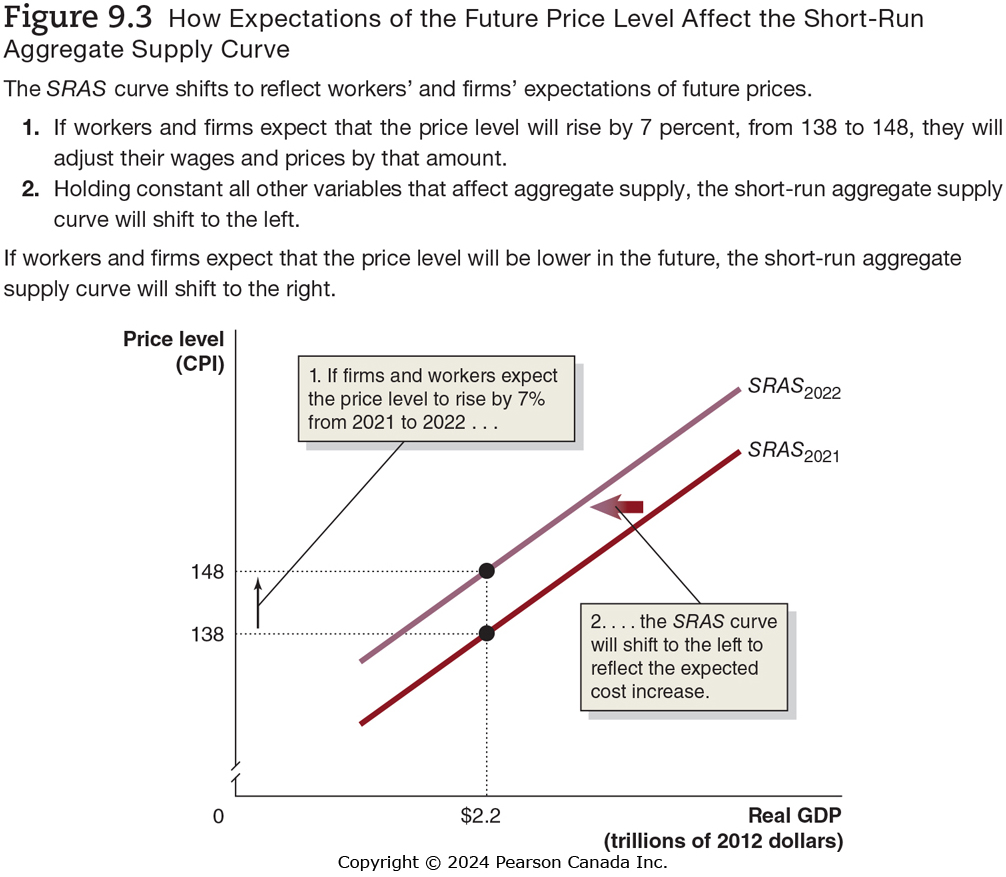
\includegraphics[width=0.57\linewidth]{Fig09-003}
\end{frame}

% ------------------------------------------------------------
% Table 9.2 Variables That Shift SRAS
% ------------------------------------------------------------

\begin{frame}{Table 9.2 -- Variables That Shift SRAS (1 of 3)}
\transfade
\begin{block}{Changes in Labour, Capital, and Technology}
\end{block}
\begin{table}[h]
\centering
\begin{tabular}{p{0.45\linewidth} p{0.45\linewidth}}
\toprule
\textbf{Change} & \textbf{Effect on SRAS} \\
\midrule
Increase in the labour force or capital stock & More production possible at any price level; \textbf{SRAS shifts right}. \\
Decrease in the labour force or capital stock & Less production possible at any price level; \textbf{SRAS shifts left}. \\
Improvements in technology & Higher productivity; more output at any price level; \textbf{SRAS shifts right}. \\
\bottomrule
\end{tabular}
\end{table}
\end{frame}

\begin{frame}{Table 9.2 -- Variables That Shift SRAS (2 of 3)}
\transfade
\begin{block}{Changes in Expectations about the Price Level}
\end{block}
\begin{table}[h]
\centering
\begin{tabular}{p{0.45\linewidth} p{0.45\linewidth}}
\toprule
\textbf{Change} & \textbf{Effect on SRAS} \\
\midrule
Workers and firms expect a higher future price level & They set higher wages and prices now; \textbf{SRAS shifts left}. \\
Workers and firms realize they previously underestimated the price level & They adjust wages and prices upward; \textbf{SRAS shifts left}. \\
Workers and firms expect a lower future price level & They accept lower wages and prices; \textbf{SRAS shifts right}. \\
\bottomrule
\end{tabular}
\end{table}
\end{frame}

\begin{frame}{Table 9.2 -- Variables That Shift SRAS (3 of 3)}
\transfade
\begin{block}{Supply Shocks}
\end{block}
\begin{itemize}[<+->]
  \item \textbf{Supply shock:}
  \begin{itemize}[<+->]
    \item Unexpected event that causes SRAS to shift.
  \end{itemize}
\end{itemize}
\begin{table}[h]
\centering
\begin{tabular}{p{0.45\linewidth} p{0.45\linewidth}}
\toprule
\textbf{Shock} & \textbf{Effect on SRAS} \\
\midrule
Unexpected increase in the price of an important input (e.g., oil) & Raises production costs; \textbf{SRAS shifts left}. \\
Unexpected decrease in the price of an important input & Lowers production costs; \textbf{SRAS shifts right}. \\
Pandemic shutdowns that close businesses & Reduce available supply; \textbf{SRAS shifts left}. \\
\bottomrule
\end{tabular}
\end{table}
\end{frame}

% ============================================================
\section{9.3 Macroeconomic Equilibrium in the Long Run and the Short Run}
% ============================================================

\begin{frame}{9.3 Learning Objective}
\transfade
\begin{block}{Goal}
Use the AD--AS model to illustrate the difference between short-run and long-run macroeconomic equilibrium.
\end{block}
\begin{itemize}[<+->]
  \item We now bring together:
  \begin{itemize}[<+->]
    \item the aggregate demand curve,
    \item the short-run aggregate supply curve,
    \item and the long-run aggregate supply curve.
  \end{itemize}
\end{itemize}
\end{frame}

\begin{frame}{Long-Run Macroeconomic Equilibrium}
\transfade
\begin{itemize}[<+->]
  \item \textbf{Long-run macroeconomic equilibrium} occurs when:
  \begin{itemize}[<+->]
    \item AD and SRAS intersect at the LRAS level of output.
  \end{itemize}
  \item That is:
  \begin{itemize}[<+->]
    \item real GDP equals potential (full-employment) GDP, and
    \item firms and workers have correctly anticipated the price level.
  \end{itemize}
\end{itemize}
\end{frame}

\begin{frame}{Figure 9.4 -- Long-Run Macroeconomic Equilibrium}
\centering
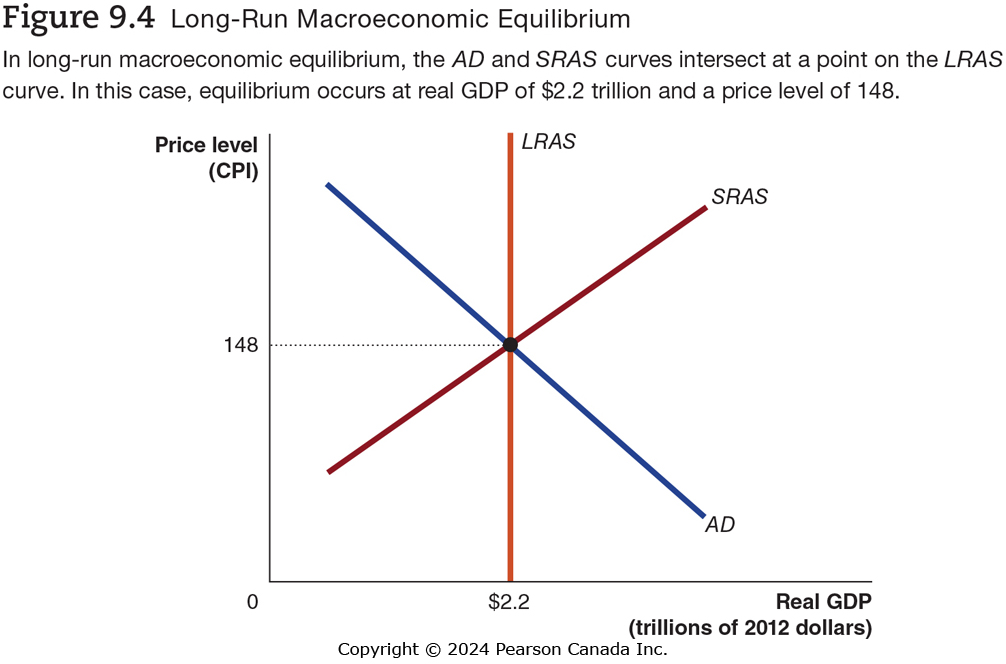
\includegraphics[width=0.7\linewidth]{Fig09-004}
\end{frame}

\begin{frame}{Why Equilibrium Occurs at Potential GDP in the Long Run}
\transfade
\begin{itemize}[<+->]
  \item Suppose the economy starts at long-run equilibrium:
  \begin{itemize}[<+->]
    \item price level \(P = 148\),
    \item real GDP \(= \$2.2\) trillion,
    \item expected future price level \(= 148\),
    \item LRAS fixed at \$2.2 trillion.
  \end{itemize}
  \item We will see how various shocks move the economy away from this point in the short run, and how the economy returns to potential GDP in the long run as wages and prices adjust.
\end{itemize}
\end{frame}

% ------------------------------------------------------------
% Figure 9.5 Decrease in AD
% ------------------------------------------------------------

\begin{frame}{Figure 9.5 -- Decrease in AD: Short Run }
\centering
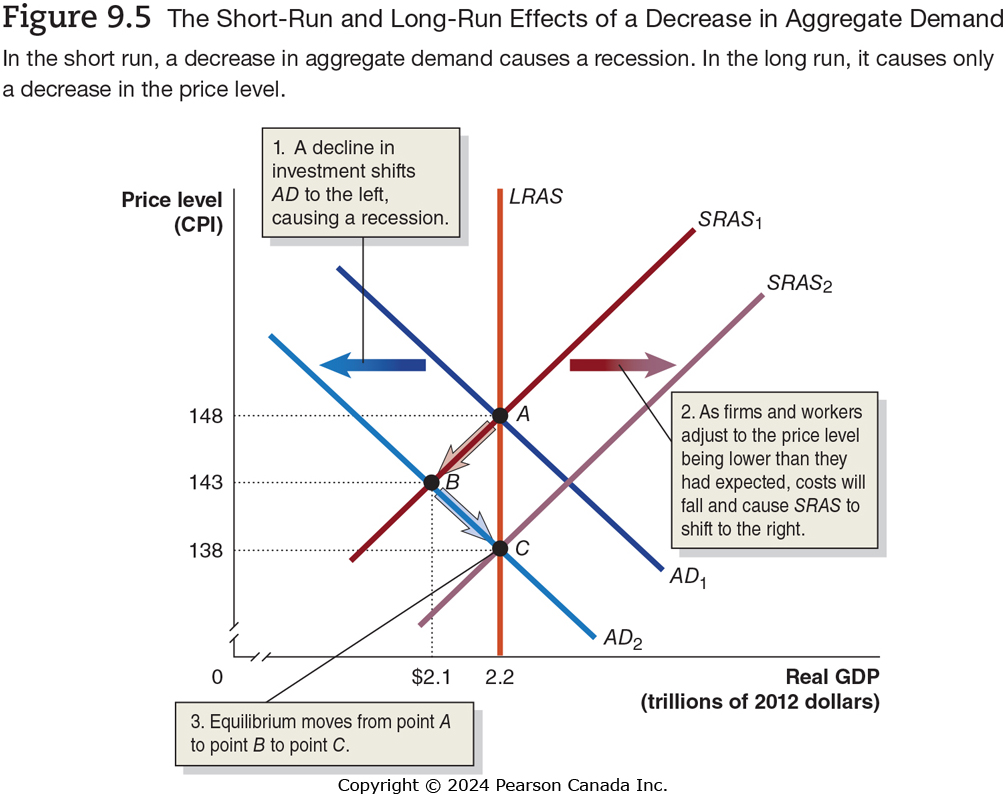
\includegraphics[width=0.64\linewidth]{Fig09-005}
\end{frame}

\begin{frame}{Short-Run Effects of a Decrease in Aggregate Demand}
\transfade
\begin{itemize}[<+->]
  \item Suppose interest rates rise (e.g., due to tighter monetary policy).
  \item Consequences:
  \begin{itemize}[<+->]
    \item Firms and households reduce planned investment.
    \item Aggregate demand shifts left (from AD\(_1\) to AD\(_2\)).
  \end{itemize}
  \item Short run:
  \begin{itemize}[<+->]
    \item real GDP falls below potential,
    \item unemployment rises,
    \item the price level falls from 148 to a lower value.
  \end{itemize}
\end{itemize}
\end{frame}

\begin{frame}{Figure 9.5 -- Decrease in AD: Long Run}
\centering
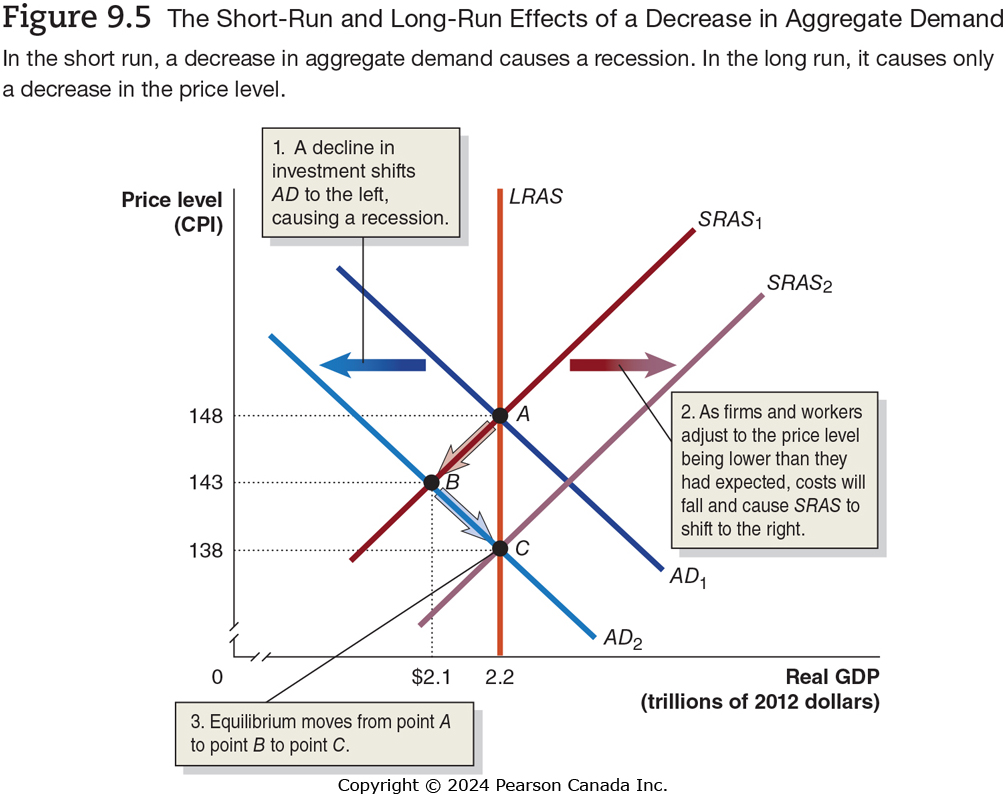
\includegraphics[width=0.64\linewidth]{Fig09-005}
\end{frame}

\begin{frame}{Long-Run Adjustment after a Decrease in AD}
\transfade
\begin{itemize}[<+->]
  \item With output below potential:
  \begin{itemize}[<+->]
    \item unemployment is higher than the natural rate,
    \item workers are willing to accept lower wages,
    \item firms anticipate lower input prices.
  \end{itemize}
  \item Over time:
  \begin{itemize}[<+->]
    \item nominal wages and other input prices fall,
    \item SRAS shifts to the right,
    \item real GDP rises back to potential.
  \end{itemize}
  \item Long-run result:
  \begin{itemize}[<+->]
    \item the economy returns to potential GDP,
    \item but the price level is lower than initially.
  \end{itemize}
\end{itemize}
\end{frame}

% ------------------------------------------------------------
% Figure 9.6 Increase in AD
% ------------------------------------------------------------

\begin{frame}{Figure 9.6 -- Increase in AD: Short Run }
\centering
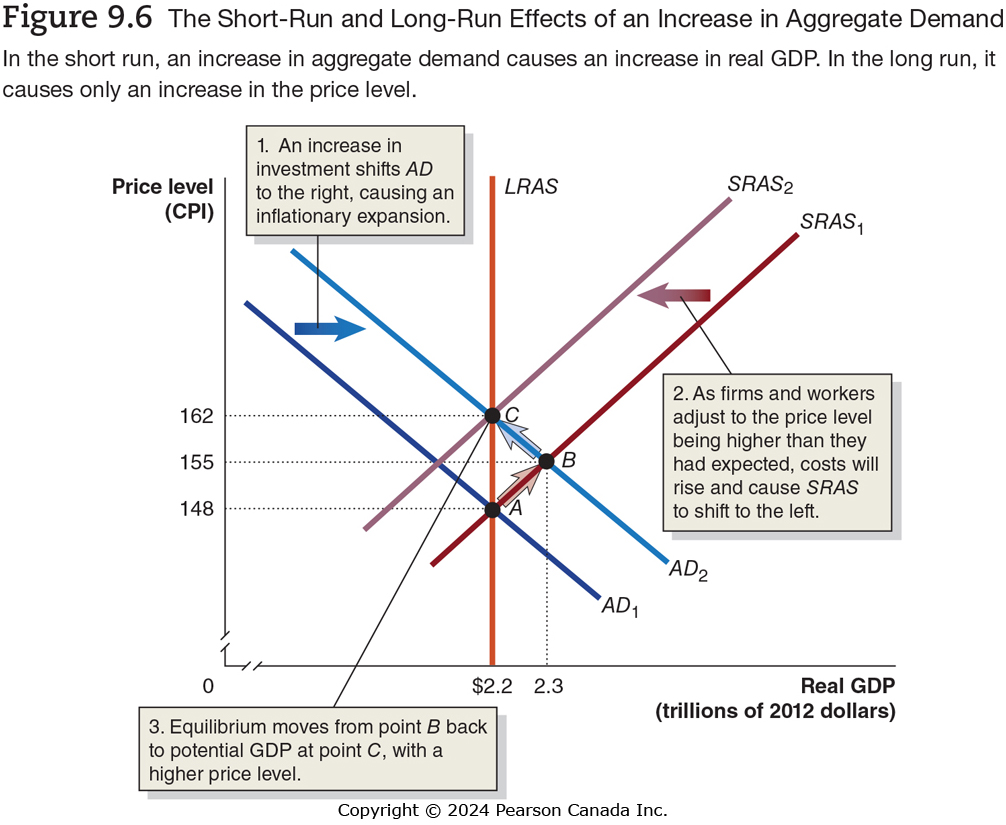
\includegraphics[width=0.62\linewidth]{Fig09-006}
\end{frame}

\begin{frame}{Short-Run Effects of an Increase in Aggregate Demand}
\transfade
\begin{itemize}[<+->]
  \item Suppose firms become more optimistic about the future.
  \item They increase their investment, shifting AD to the right (from AD\(_1\) to AD\(_2\)).
  \item Short run:
  \begin{itemize}[<+->]
    \item real GDP rises above potential,
    \item unemployment falls below the natural rate,
    \item the price level rises.
  \end{itemize}
\end{itemize}
\end{frame}

\begin{frame}{Figure 9.6 -- Increase in AD: Long Run }
\centering
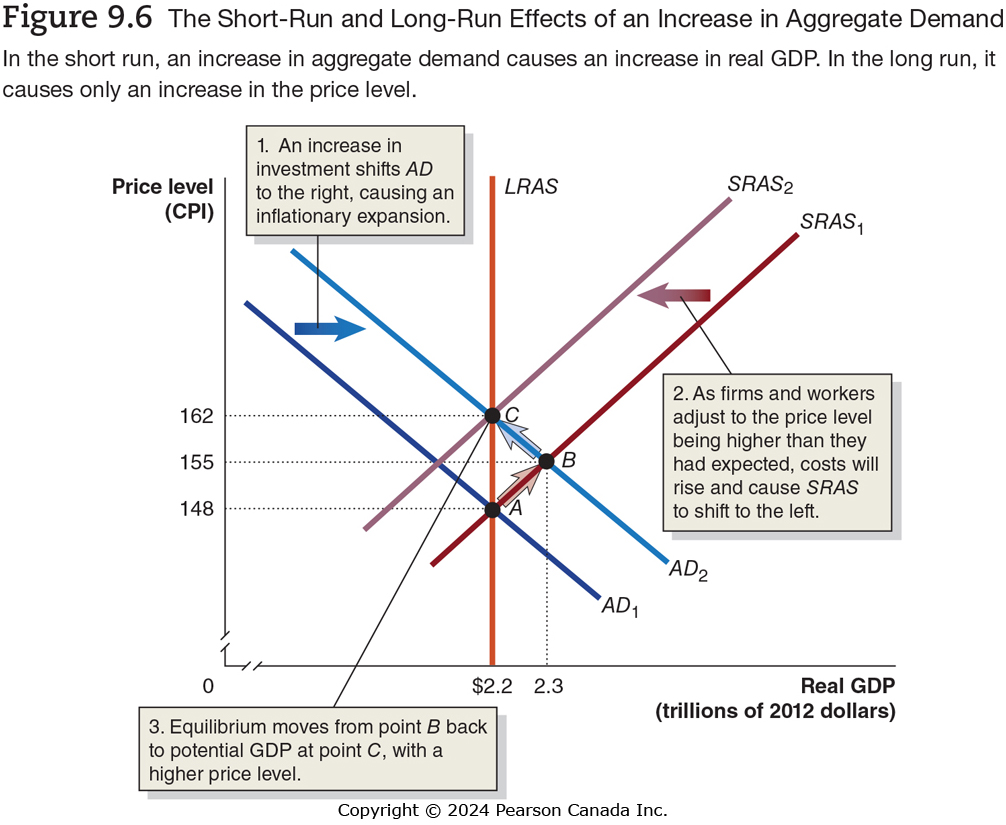
\includegraphics[width=0.62\linewidth]{Fig09-006}
\end{frame}

\begin{frame}{Long-Run Adjustment after an Increase in AD}
\transfade
\begin{itemize}[<+->]
  \item With output above potential:
  \begin{itemize}[<+->]
    \item labour markets are tight,
    \item firms bid up wages to attract workers,
    \item higher demand for goods and services supports higher prices.
  \end{itemize}
  \item Over time:
  \begin{itemize}[<+->]
    \item expectations of the price level rise,
    \item wages and input prices increase,
    \item SRAS shifts left.
  \end{itemize}
  \item Long-run result:
  \begin{itemize}[<+->]
    \item the economy returns to potential GDP,
    \item but the price level is higher than initially.
  \end{itemize}
\end{itemize}
\end{frame}

% ------------------------------------------------------------
% Figure 9.7 Supply Shock
% ------------------------------------------------------------

\begin{frame}{Figure 9.7 -- Supply Shock: Short Run }
\centering
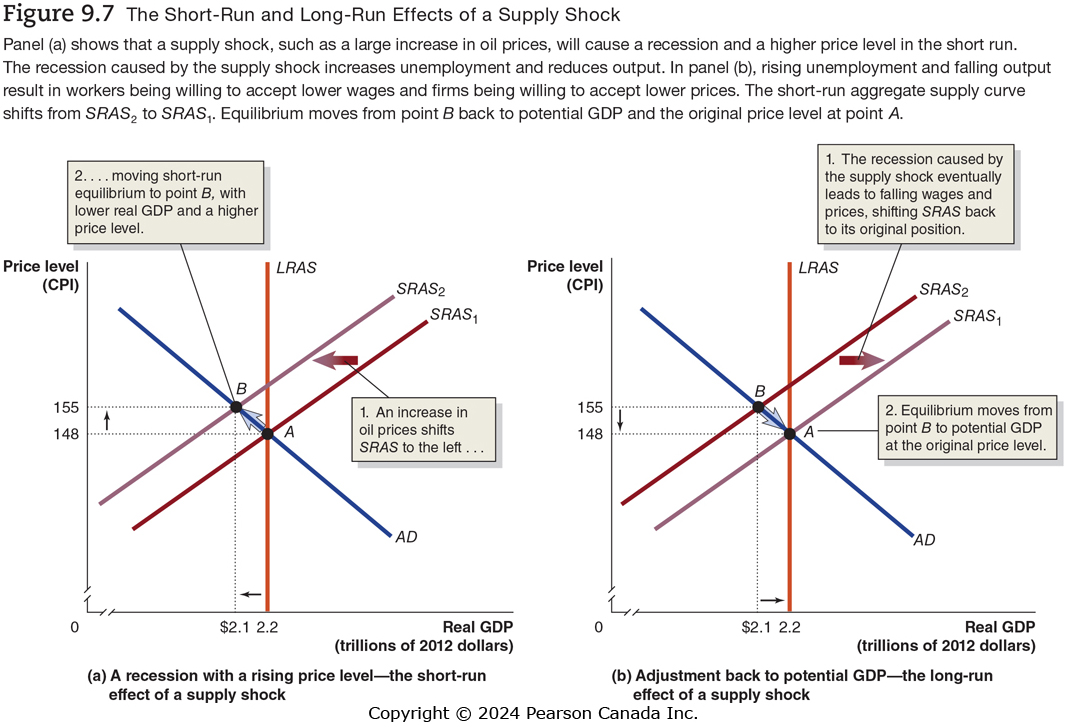
\includegraphics[width=0.65\linewidth]{Fig09-007}
\end{frame}

\begin{frame}{Negative Supply Shock and Stagflation}
\transfade
\begin{itemize}[<+->]
  \item \textbf{Supply shock:}
  \begin{itemize}[<+->]
    \item Unexpected event that causes SRAS to shift.
  \end{itemize}
  \item Example: a sudden increase in oil prices.
  \item Short-run effects:
  \begin{itemize}[<+->]
    \item SRAS shifts left,
    \item real GDP falls,
    \item unemployment rises,
    \item price level rises.
  \end{itemize}
  \item This combination of \textbf{inflation} and \textbf{recession} is called \textbf{stagflation}.
\end{itemize}
\end{frame}

\begin{frame}{Figure 9.7 -- Supply Shock: Long-Run Adjustment}
\centering
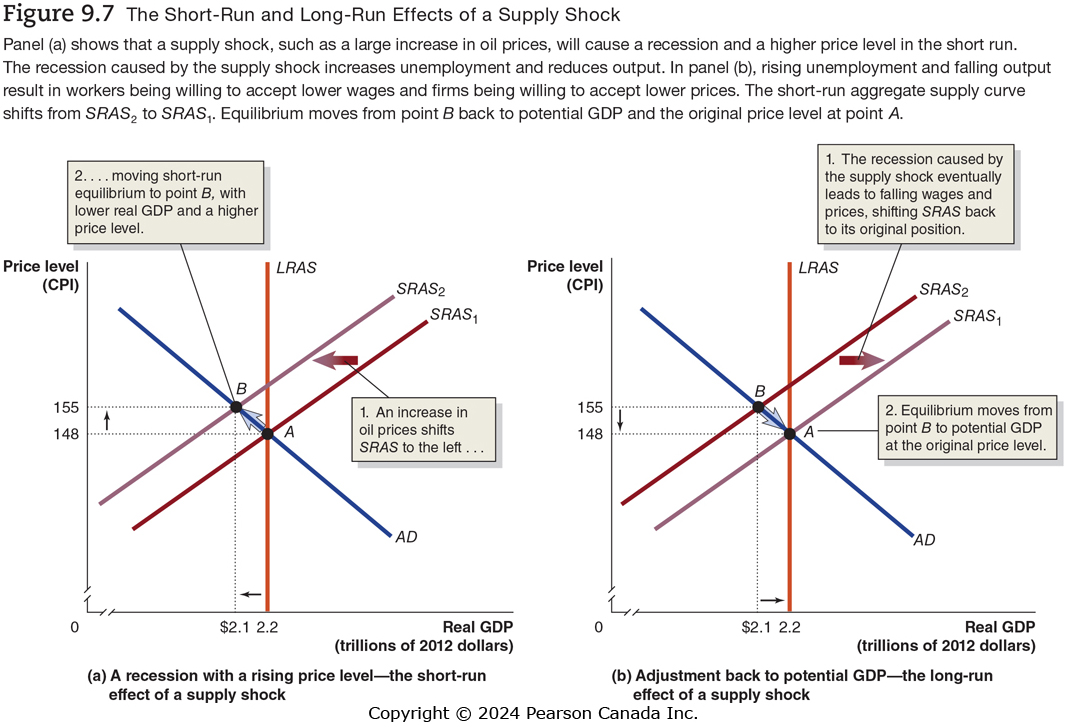
\includegraphics[width=0.65\linewidth]{Fig09-007}
\end{frame}

\begin{frame}{Long-Run Adjustment after a Supply Shock}
\transfade
\begin{itemize}[<+->]
  \item With output below potential and high unemployment:
  \begin{itemize}[<+->]
    \item workers are willing to accept lower wages,
    \item firms reduce prices to clear inventories.
  \end{itemize}
  \item As expectations of future prices fall:
  \begin{itemize}[<+->]
    \item SRAS shifts right again.
  \end{itemize}
  \item Eventually:
  \begin{itemize}[<+->]
    \item the economy returns to potential GDP,
    \item and the price level may fall back toward its initial value.
  \end{itemize}
\end{itemize}
\end{frame}

\begin{frame}{Figure 9.7 -- Policy Response to Supply Shocks}
\centering
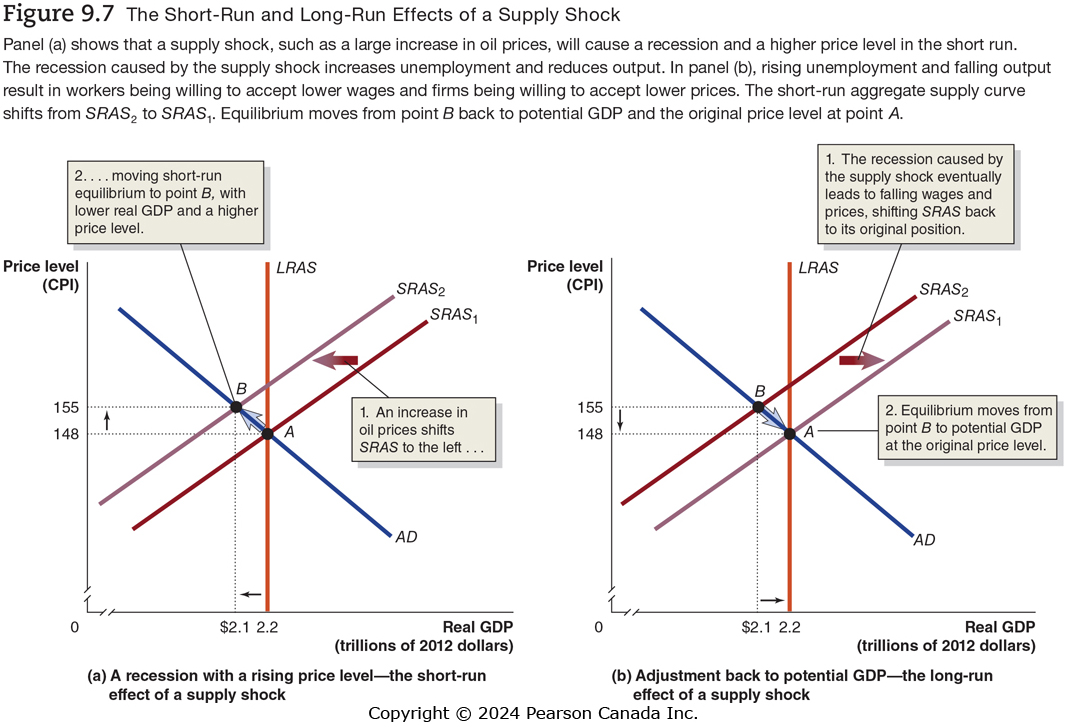
\includegraphics[width=0.65\linewidth]{Fig09-007}
\end{frame}

\begin{frame}{Policy Trade-Offs after a Supply Shock}
\transfade
\begin{itemize}[<+->]
  \item Left alone, the economy eventually returns to full employment, but:
  \begin{itemize}[<+->]
    \item it may take several years,
    \item unemployment can remain high for a long time.
  \end{itemize}
  \item Policymakers may choose to:
  \begin{itemize}[<+->]
    \item use fiscal or monetary policy to increase AD,
    \item reducing the depth and length of the recession,
    \item but at the cost of permanently higher price levels.
  \end{itemize}
\end{itemize}
\end{frame}

% ------------------------------------------------------------
% Apply the Concept: COVID-19 Recession
% ------------------------------------------------------------

\begin{frame}{Apply the Concept: COVID-19 -- Supply Shock or Demand Shock? (1 of 3)}
\transfade
\begin{itemize}[<+->]
  \item Both supply and demand shocks can cause recessions.
  \item Question: \emph{Which type of shock played a larger role in the 2020 COVID-19 recession?}
  \item A \textbf{negative supply shock}:
  \begin{itemize}[<+->]
    \item closes businesses,
    \item reduces productive capacity,
    \item shifts SRAS left,
    \item reduces output and raises prices.
  \end{itemize}
\end{itemize}
\end{frame}

\begin{frame}{Apply the Concept: COVID-19 -- Supply vs. Demand (2 of 3)}
\transfade
\begin{itemize}[<+->]
  \item A \textbf{negative demand shock}:
  \begin{itemize}[<+->]
    \item reduces household and business demand for goods and services,
    \item shifts AD left,
    \item reduces output and lowers prices.
  \end{itemize}
  \item In either case:
  \begin{itemize}[<+->]
    \item real GDP falls,
    \item recession occurs.
  \end{itemize}
\end{itemize}
\end{frame}

\begin{frame}{Apply the Concept: COVID-19 -- Evidence from 2020 (3 of 3)}
\transfade
\begin{itemize}[<+->]
  \item In the first half of 2020:
  \begin{itemize}[<+->]
    \item Real GDP fell from about \$2.12 trillion at the end of 2019
    \item to about \$1.85 trillion by mid-2020.
  \end{itemize}
  \item Consumer prices:
  \begin{itemize}[<+->]
    \item The seasonally adjusted CPI was 137.3 in January 2020.
    \item It was 136.7 in July 2020, when output had started to recover.
  \end{itemize}
  \item Prices \textbf{fell} during the recession:
  \begin{itemize}[<+->]
    \item This pattern is more consistent with a \textbf{demand shock} than with a pure supply shock.
    \item Conclusion: a fall in aggregate demand played a larger role in the 2020 recession, though supply disruptions also mattered.
  \end{itemize}
\end{itemize}
\end{frame}

% ============================================================
\section*{Chapter Summary}
% ============================================================

\begin{frame}{Summary}
\transfade
\begin{itemize}[<+->]
  \item The \textbf{aggregate demand curve} slopes downward because:
  \begin{itemize}[<+->]
    \item a higher price level reduces consumption (wealth effect),
    \item reduces investment (interest-rate effect),
    \item and reduces net exports (international-trade effect).
  \end{itemize}
  \item Changes in government policy, expectations, and foreign variables shift AD.
  \item The \textbf{long-run aggregate supply} curve is vertical at potential GDP; the \textbf{short-run aggregate supply} curve is upward sloping due to sticky wages and prices.
  \item Long-run equilibrium occurs where AD and SRAS intersect LRAS.
  \item Demand shocks shift AD; supply shocks shift SRAS. Both can cause recessions, but with different inflation patterns.
\end{itemize}
\end{frame}

\begin{frame}
\centering
\Huge \textbf{Thank you!}
\end{frame}

\end{document}
